\section{SunDog Interior}

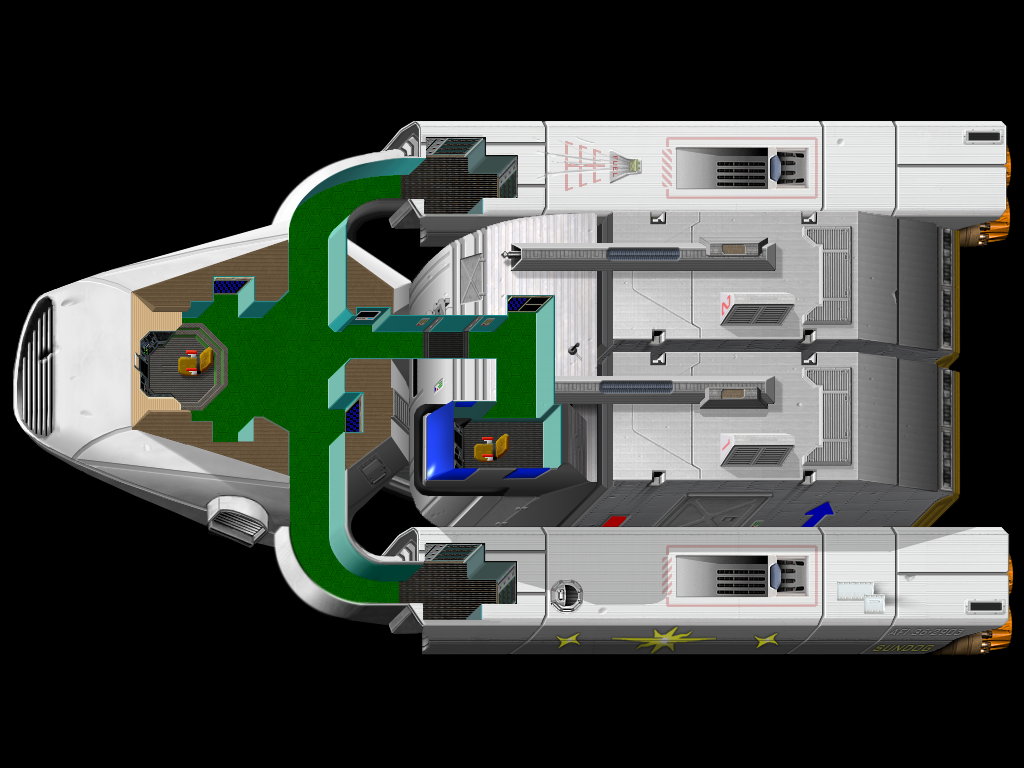
\includegraphics[scale=0.35]{images/sundog-interior-with-pod.png}



TODO:
\begin{itemize}
\item add sundog interior image without the pod
\end{itemize}

\subsection{Collision Detection}


\includegraphics[scale=0.35]{images/sundog-interior-with-pod-collidemap.png}

\subsection{Cockpit}

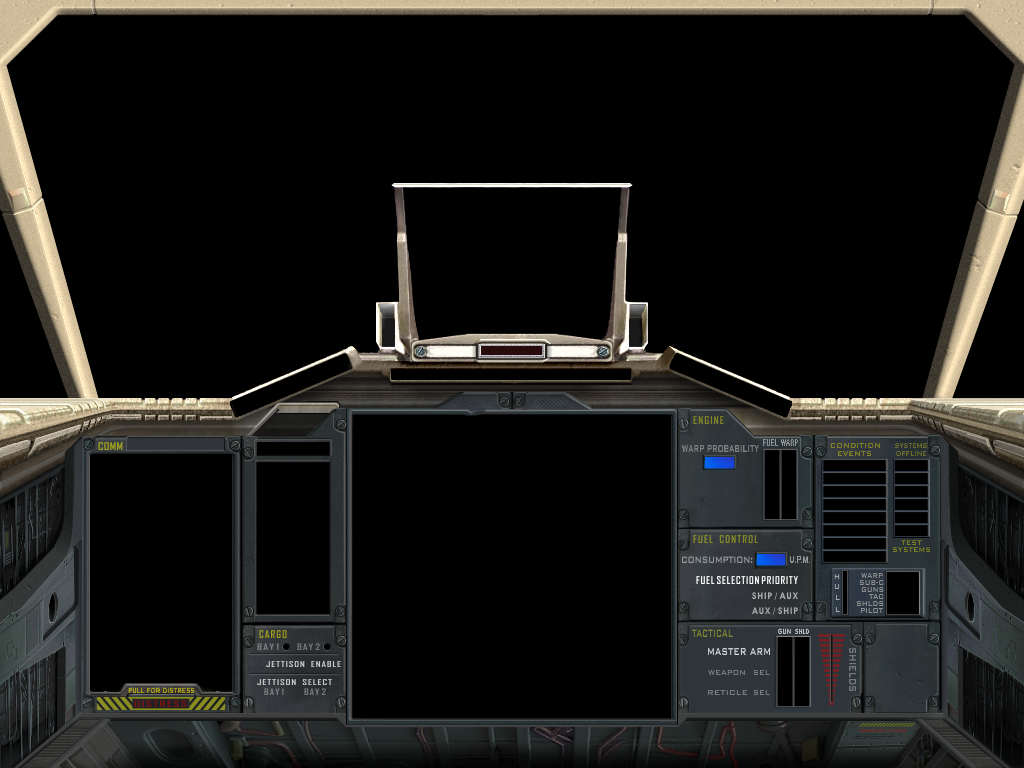
\includegraphics[scale=0.35]{images/cockpit.png}

The cockpit of the SunDog is the command center for the entire ship.  At
first the cockpit, like that of an airplane, can look like a fairly daunting
place, however, the controls are grossly simplified and should be fairly
easy to figure out.

\subsubsection{Comm}
The Comm system is used for ship-to-ship communications, and possibly, to
play music on "radio stations" broadcast from planets that are within range
of the Sundog.  

The comm control panel has five channels, one per button. The buttons are
located in the indented strip at the top of the panel.

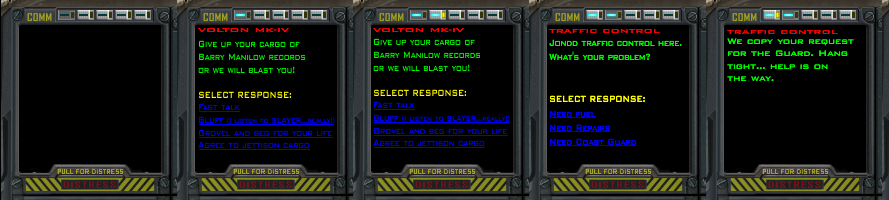
\includegraphics{images/beta COMM storyboard.png}

The comm is inactive until it receives a signal. The user can hit any of the
five buttons at any time, depressing the button as is shown in comm screen
#1 (far left) but nothing will show on the screen if there is no signal.
(alternatively, we can have a short message like "Channel 1 - No uplink"
display on the comm screen if the player pushes buttons without a signal.)

When a signal is received, it is funneled into the first unused channel - in
the storyboard's case, it is the first button. When the signal comes, it
lights up the button with a blue line, to show this is an active channel. An
alert sound should accompany the initiation of the signal. The blue bar on
the button will light up regardless of whether the channel button is
currently depressed or not. (see screen #2 in the storyboard).

The message displays in the screen, with the source at the top, followed by
the source's message, then by the options (like hyperlinks) for the user to
select. The NPC ship replies or updates the information due to the player's
non-response, and the player is given new options to respond with. Such
time-out for non-response should be 30 seconds. If the player does not click
one of the options within 30 seconds (regardless of whether the channel
screen is visible or not) the NPC will send another message or terminate the
conversation and begin shooting. (re: original game)

If during the course of the first radio conversation a second one is
initiated or received, the next available comm channel button will light up
blue. Moreover, it will also have a blinking yellow light, that will blink
twice a second.  (See screen #3 in the storyboard). The yellow light
indicates that there is an unread message on that screen.

Pushing the second channel button will switch the screen to that conversation.
(See screen #4). The blinking yellow light turns out, as you now have
displayed the new message. Note both channels, including the first, are lit
blue, as they both have active conversations.

If during the course of the second conversation a message is received in the
first conversation, the yellow light will begin to blink, indicating the new
message. (see screen #5). It will continue to blink until the player switches
back to that conversation.

Once a conversation is concluded, a text message should indicate this
(i.e. "Uplink terminated") at the bottom of the screen under the text of the
last message, and the blue light will turn off. When the user leaves the
screen for another, the text (containing the NPC's last message) on the
screen will be lost, and a blank screen will result if the player returns to
that screen.

If a conversation terminates while the player is viewing another screen, the
yellow light will blink (just as if it received a new message) and when the
player changes to that channel they will see the last message and the text
alert indicating the conversation is over.

The DISTRESS bar will activate if the player clicks it, and it will open a
conversation with traffic control. Once clicked, the bar should remain down
and lit up. After traffic control answers and then concludes the conversation
(either with the player requesting help or a time-out where the player never
requests anything), the distress bar should automatically spring back into
place. The timeout should be 30 seconds, where if the TC answers and the
player doesn't choose an option in 30 seconds, the TC will terminate the
conversation.

Color scheme for text:
Red = source name and system alerts (i.e. "lost uplink", "message terminated",
etc)
Green = NPC message
Yellow = Player Prompt
Blue = Player's response


MUSIC: 
For the music radio broadcast, it will work just like an incoming
conversation described above, with the exception that the yellow light will
never flash as it is assumed the radio broadcast is constant, regardless of a
song change, etc. When the player nears a planet and is within radio range,
they a channel button will light up. The comm screen will then act as a
browser that will let the player switch tunes, review information, etc. This
spec will be drawn up later on  (I don't expect us to worry about radio
stations for a while - we have bigger fish to fry first). When the player
leaves the range of the station, it will terminate and the screen will go
blank.


\begin{tabular}{ | l | l | l | }
\hline
Indicator or Button & Active & Inactive \\
\hline
Distress & 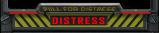
\includegraphics[scale=0.5]{images/distress_on.png} & 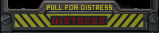
\includegraphics[scale=0.5]{images/distress_off.png} \\
\hline
\end{tabular}

DISTRESS 

The player can make a distress call by clicking on the DISTRESS bar at the bottom of the COMM. Upon click, the bar's image will change from the "OFF" version to the "ON" version, and the COMM screen will then display the interaction between the player and the dispatcher of the local planet. 

When the distress call is answered by the dispatcher, the interraction takes place similar to a call to 911. Upon pulling the distress handle, the dispatcher sends a message asking the nature of the problem, and gives options for the user to choose. The user may choose multiple items from the list. The options should include: 
NEED FUEL - Dispatcher then sends a fuel tanker to the ship's location. Upon arrival, the Sundog's on board tank is filled to 100%. Cost for this procedure is based on the local cost of a full load fuel bought at the space port, times three. 
NEED RESCUE - Dispatcher will send the planetary coast guard to chase the pirates away and escort the ship. The player will wait (just like for fuel) until the Guard arrives, upon which if the player is still alive, the pirates will flee. Player can then continue on to the planet under guard. The player may preemptively call the Guard if he knows the system is bad and he has a high chance of being attacked. However, the cost of this procedure should make preemptive calls for the Guard cost-prohibitive.
NEED TOW - Dispatcher will send a tow "truck" to Sundog's location and tow it to the nearest planet's spaceport. This option may be employed if the ship is so badly damaged that even with fuel it cannot operate under its own power. The cost of this tow should be a base price plus an amount that reflects the distance of the tow. 

The response time between the distress call and the arrival of help will vary. The response time depends on three factors: Distance from closest planet (from where the rescue is coming), Lawlessness, and Population of Planet. A slight randomizing factor should be included so no two response times in the same system are exactly the same. 
 
Distance: measure the distance between the ship and the closet inhabited planet (presumably the to which you are traveling). The longer the distance, the longer the wait. For example, a 3 AU distance would mean 6 real-world minutes of wait time, while a 0.5 AU would mean a 1 minute wait. This equation is purely for demonstration - a real equation can be created when we determine the units of measurement that will be used in the game. 

Lawlessness: In systems with lots of pirate activity, rescue might be sporadic, much as an ambulance arrival might be unpredictable in the deep ganglands of Detroit. The higher the level of lawlessness, the longer the delay. For example, for each lawlessness variable level (rated from 1-10) add 30 seconds. 

Population: In a heavily populated system, there will be a large social infrastructure to handle distress calls in the busy space of traffic lanes. Thus response time will be decreased. In small or new colonies, there might be one battered rescue ship on standby, which will increase response time. Example: a median population factor (5) will not affect response time. For each variable factor over 5, decrease response time by 15 seconds. For each factor below 5, add 15 seconds. 

Open Items:
\begin{itemize}
\item  Can we show multiple conversations on the Comm display?
the cursor up similar to the sliders?
\end{itemize}

\subsubsection{Tactical}
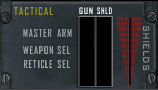
\includegraphics[scale=0.7]{images/tactical.png}

The tactical panel controls the weapons and shields systems of the SunDog.
Arming the tactical controls can be done by toggling either the "Master Arm"
button, or the "Nav/Tac" button just below the HUD.  Tactical mode can
only be entered when the SunDog is in space.

In tactical mode, the ship will yaw or pitch along with the mouse.  If
the mouse moves up, the nose of the ship will pitch down, and conversely
if the mouse moves down, the nose of the ship will pitch up.  If the
mouse is moved to the left or right, it will yaw the SunDog in either
of those directions.  The further the mouse is moved, the more the ship
will pitch or yaw.  The ship will continue to move in the same direction until
the reverse action is done (there is no friction in space!).  If the
ship is pitching upward, the mouse must be moved upward to pitch the nose
down.

The "Weapons Sel" button toggles between the ships cannon and its laser, 
which is displayed on the HUD.

When the "Reticle Sel" button is pressed the reticle on the HUD will
illuminate and stay lit for 3 seconds.  If the button is pressed again
before the reticle disappears, it will cycle to the next reticle
in the sequence.  The time that the reticle stays illuminated will
be reset to 3 seconds.

The "Gun" status indicator shows the charge of the currently selected
weapon system.  A "peak" mark will be displayed at the highest amount
the guns can charge to.  The guns status indicator will normally be in
green, however if concentrators are used the value can go past 100\%.
In this case, values above 100\% will be shown as a secondary bar in
red which overlaps the primary bar.

In the event the player has installed "concentrators" into the gun bay (special parts bought on the black market that increase gun strength), the gun strength can increase above the normal 100%. Each concentrator adds 25% power bonus on the existing gun strength. Without concentrators, the gun indicator bar is a dark red. When concentrators are installed and the gun charges to the new max charge, the additional 25% (or 50%, 75%, etc) will be indicated by a second, overlapping bar of bright red that should start at the bottom of the indicator bar and rise until it hits the maximum. So if one concentrator is installed and the user turns on the guns (or if the gun is fired, sending the gun charge down to 0%), the dark red bar will rise to 100% as it charges, from bottom to top, and then a bright red bar will rise, starting from the bottom and obscuring the existing dark red bar, and it will rise to 1/4 the height of the indicator bar (25%). Please note that this assumes all four rails in the Gun bay are fully functioning. If there is a dead rail or shunts are used, the maximum gun power will be reduced accordingly. 

The "SHLD" status indicator shows the current charge of the shields and
the SHIELDS slider bar can be moved to turn on a dynamic ount of
shield power.  A "peak" mark will be displayed at the highest amount
the shields can charge to, which the shields will not charge past
even if the slider is set higher.

Art Assets:

\begin{tabular}{ | l | l | l | l | }
\hline
Indicator or Button & Active & Inactive & Misc\\
\hline
Master Arm & 
\includegraphics{images/button_danger_on.png} & 
\includegraphics{images/button_danger_off.png} & \\
Weapon Sel & 
\includegraphics{images/button_on.png} & 
\includegraphics{images/button_off.png} & \\
Reticle Sel & 
\includegraphics{images/button_on.png} & 
\includegraphics{images/button_off.png} & \\
Shields & & & 
\includegraphics{images/slider.png} \\
Gun Gauge & (255, 0, 0, 255) & & \\
Shield Gauge & (255, 0, 255, 255) & & \\
\hline
\end{tabular}

Open Items:
\begin{itemize}
\item We need to include a table of reticles that the user can cycle through.
\item If the shields can only work at a reduced efficiency, do they still
take the same amount of fuel to run as they would if they were 100\%?
\item The buttons are somewhat small, so do we want it to toggle them
when a user clicks on the writing as well as the button?
\end{itemize}

\subsubsection{Cargo}

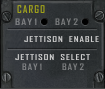
\includegraphics[scale=0.7]{images/cargo.png}

Sometimes during ship to ship fighting it becomes necessary to jettison cargo.
The "BAY 1" and "BAY 2" status lights are illuminated green (0, 255, 0, 255)
whenever cargo is present in its respective bay.  To eject cargo, the
"Jettison Enable" button must be toggled to the on position, which will
illuminate the "Jettison Select" buttons for whichever bay currently
has cargo.

After pushing a "Jettison Select" button, the cargo bay light will no longer
be illuminated and the jettison select button will become inactive.  The
indicator light should fade from green to black in 1\slash 4 of a second.

Art Assets:

\begin{tabular}{ | l | l | l | p{3.5cm} | }
\hline
Indicator or Button & Active & Inactive & Notes \\
\hline
Enable Button & 
\includegraphics{images/button_red_on.png} & 
\includegraphics{images/button_red_off.png} & \\
Jettison Select & 
\includegraphics{images/button_danger_on.png} & 
\includegraphics{images/button_danger_off.png} & \\
Bay Lights & (0, 255, 0, 255) & & The indicator should fade in or out whenever
cargo is ejected or picked up (usually by the tractor beam) \\ 
\hline
\end{tabular}

Open Items:
\begin{itemize}
\item Do we want the status light to fade out or just go 
\end{itemize}

\subsubsection{Heads Up Display}

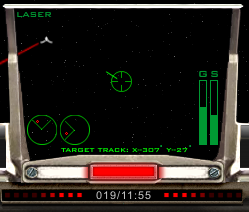
\includegraphics[scale=0.7]{images/hud.png}

The heads up display (HUD) is the main tactical viewport of the Sun Dog.  When
tactical mode is activated, the HUD will illuminate its center targeting reticle
and the tracking "radar" circles for fighting enemy ships, both located in the lower left of the HUD.  In addition, tracking information is displayed in the lower portion of the view port: X, Y, and Z coordinates. Gun and Shield strength bars are shown in the lower right side. This is redundant with the primary controls on the dashboard, but in a firefight it will be helpful to have this critical information immediately adjacent to the action. If redundancy was to be avoided, the classic control panel would have to be removed and redrawn, OR the handy HUD status bars would not be used. Considering the Sundog is an inelegant, clunky freighter, it seems natural that some redundancy would occur. The currently selected weapon will be displayed in the upper left hand corner as text (i.e. Laser, cannon, etc). A small "pointer" can indicate the direction of the enemy ship. Current fighter jets have such a feature, and it would make sense such a feature would be available in the future. (This feature is not critical, and can wait for future versions of the game). 

Everything in the HUD is to be drawn programatically. 

Warp effects: The original game had a "Star Wars" style warp effect. A similar effect should be employed in this version of the game. The predominant color of the stars in the effect should be shades of gray, with some colored stars lightly employed. The warp effect should start with the present starfield moving slowly towards the cockpit, some stars moving faster due to their close proximity. The sound of engines rev, and the stars move faster until they begin shooting at the cockpit, multiplying until they fill the entire blackness of space with light. Another effect of "hyperspace" should then appear, followed by a sudden cessation of star motion and returning the player to a static field of stars. 

If a raster graphic of stars is used for the background of space (which would be easiest to program and lightest on memory as opposed to a background of star-objects), it will be difficult or impossible to have a smooth transition from the background the star field to the slowly moving star field in the beginning stages of warp. To fix this problem, the ship should roll before engaging the warp engine. During the roll, the background star field should be discretely replaced with the first frame of the warp animation sequence, which is a static star field that will shortly begin to move. 

Open Issues:
\begin{itemize}

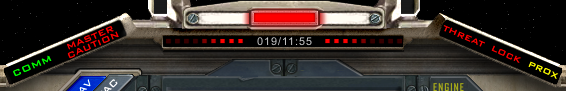
\includegraphics[scale=0.7]{images/lower-hud.png}

Below the HUD is the red alert indicator which should activate when the
SunDog is under attack.  This lights up when the ship is under attack, and an audible klaxon sounds in the background. The light will remain illuminated until the enemy ship is destroyed or flees. There is a graphic image for the "on" state of the light, which allows some reflected illumination to appear on cockpit surfaces near the light. 


A chronometer with the current game time is displayed underneath the red
alert indicator and a pulsing strip surrounds it which signals that the ships
Sub-C engines are currently activated.

A MASTER CAUTION light illuminates when a new situation occurs, such as a system failure, hull damage, etc. It will remain illuminated until the player clicks it. Upon a click, it will turn off, until another event occurs that will trigger it. 

THREAT LOCK indicates the enemy ship's weapons systems are locked onto the Sundog and that attack is imminent. In a typical engagement, this will illuminate after the dialogue between the pirates ends and just prior to the pirate ship making an attack. It will remain on until the pirate ship either begins to flee, is destroyed, or when the player jettison's the cargo and the attack ends. 

PROX is a proximity alert. It may illuminate when the pirate ship in the course of an attack gets too close. Other uses for it may be planned in the future. 

Open Issues:
\begin{itemize}
\item How does the COMM indicator work?
\end{itemize}

\subsubsection{Primary Flight Display}

Open Issues:
\begin{itemize}
\item Need to mock up the various screens for how this is going to work.
\end{itemize}

\subsubsection{Computer}

Between the COMM and the MFD there is a NAV-TAC menu panel. This panel has a tabbed button at the top. The default mode is NAV for Navigation. In this mode, the menu will display appropriate text options for commands, such as TAKE OFF, LAND, MAPS, etc. When the player selects the TAC tab, the ship enters "Tactical Mode" and tactical menu options are now displayed in the menu. These tabs work just like the original game, which contained a NAVIGATION and TACTICAL button on the screen. Pressing either button, just as pressing the tabs here, will bring up a menu of options. While on the ground, the TAC menu is inaccessible and clicking on the TAC tab will result in a beep and a text message on the MFD saying "TACTICAL MODE NOT AVAILABLE WHILE ON GROUND".

NAV Menu options are as follows: 
On the ground:
- LIFTOFF
- SET WARP
- MAPS
- CITY-CITY (when a ground scanner is installed)

In orbit or in flight:
- LAND (if orbiting)
- SUB-LIGHT
- HALT(if currently sub-lighting)
- SET WARP 
- DO WARP (warp may not be successful if it does not have a high enough probability %, and ship is not located at jump point)
- STOP WARP (if warp is charging or fully charged)
- MAPS
- SET YAW (Described below)
- SET ROLL (Described below)

There should be some way of changing ship settings such as yaw vs.
roll. This can be a menu option in the NAV menu. The menu items should be SET YAW (when ROLL is selected) and SET ROLL (when YAW is selected.) When either of these options are chosen, a text message should appear in the main MFD stating "YAW NOW SELECTED" or "ROLL NOW SELECTED". 

TAC Menu options are as follows: 
- LASER
- CANNON
- TRACTOR (Clicking this will bring in cargo jettisoned or lost during combat. Clicking it when no cargo is in range will result in a beep and a message on the MFD: "SCANNERS DETECT NO CARGO IN VICINITY FOR TRACTOR BEAM"
- CLOAK (when cloaker is installed)
- DE-CLOAK (when de-cloaker is installed)



Open Issues:
\begin{itemize}


\item We need to mock up the various situations for what menu items
will show up in the computer. 
\end{itemize}

\subsubsection{IFF}

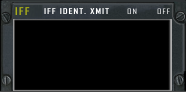
\includegraphics[scale=0.70]{images/iff.png}

When the SunDog comes across another vessel or object in space, the ship's
onboard IFF system will display information about the object.  

Art Assets:

\begin{tabular}{ | l | l | }
\hline
Ship or Visual & Image \\
\hline
Angolith MK-V & \\
Annihilator & \\
Cryn MK-90 & \\
Cryn MK-110 & \\
Cryn MK-140 & \\
Death Angel MK-2 & \\
Debris Field & \\
Jammed Signal & \\
Kolum 8820 & \\
Life Pod & \\
Gorathi M5 & 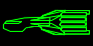
\includegraphics[scale=0.75]{images/ship_gorathi_m5.png} \\
Phantom UL & 
\includegraphics[scale=0.75]{images/ship_Phantom_UL.png} \\
Probe & \\
Rathain M1 & \\
Rathain M5 & \\
Rynroth-VOR & \\
Shath Class 3 & \\
Skryth MK-IV & 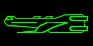
\includegraphics[scale=0.75]{images/ship_skryth_mk-iv.png} \\
Skryth MK-VII & \\
Sorth CF-50 & 
\includegraphics[scale=0.75]{images/ship_sorth_cf-50.png} \\
Space Station & \\
Space Station & \\
Unknown Enlie & \\
Valshur 85 & \\
Valshur 130 & \\
Vestar Class II & 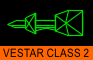
\includegraphics[scale=0.75]{images/ship_vestar_class_2.png} \\
Volton MK-IV & 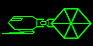
\includegraphics[scale=0.75]{images/ship_Voton_MK_IV.png} \\
Volton MK-X & 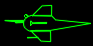
\includegraphics[scale=0.75]{images/ship_Voton_MK_X.png} \\
VW 69 & 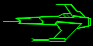
\includegraphics[scale=0.75]{images/ship_VW-69.png} \\
Z1 - Vector & \\
\hline
\end{tabular}

Enemy ships should have health ratings. (Table of health ratings to be made in future) A small, light ship might have a health rating of 200, while a heavy cruiser might have 4000. 


Open Issues:
\begin{itemize}
\item Fill in the rest of the wireframes.
\item Are certain ships more likely in certain places with less lawlessness?
\item What are the different capabilities of each of the ships?
\item It would be nice to do a rotating wireframe of each ship.
\item We need to have corresponding 3D models to each of the ship outlines.
\end{itemize}

\subsubsection{Engine}
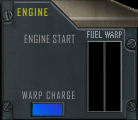
\includegraphics[scale=0.70]{images/engine.png}

Open Issues:
\begin{itemize}
\item The warp charge entry needs to be changed to the successful warp
probability meter.
\end{itemize}

\subsubsection{Fuel Control}
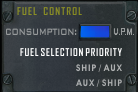
\includegraphics[scale=0.70]{images/fuelcontrol.png}

Fuel control shows the current fuel drain on the ship, and allows the player
to decide whether to draw fuel from an axillary fuel pod, or from the
ship's fuel tanks.  Fuel drain is calculated at in "Units Per Minute" for
each of the ships systems.

The "Ship\slash Aux" button in the fuel control panel will default to
being illuminated.  If there is an axillary fuel pod onboard, pressing
"Ship\slash Aux" or "Aux\slash Ship" will cause whichever button was
pressed to be illuminated and the other button to be inactive.  Otherwise
"Ship\slash Aux" will always be active.  Fuel will drain from whichever
supply is selected until it runs out, at which point it will start to drain
from the other supply.  If the "AUX\slash SHIP" button is pushed when there is no axillary
fuel pod, this is not a problem as the system will treat the lack of fuel in the AUX as if that supply had run dry, and the system will look only to the ship's tanks for fuel. 

When fuel runs out, all systems except the Comm will be inoperative and
the "Systems Offline" and "Low Fuel" indicators will become illuminated.

When the player calls for a refuel in space, a tanker will arrive after a time. (See above for details.) When the tanker arrives, an audible scraping-clunking noise is heard and the hum of fuel rushing into the ship's tank. This sound sequence lasts three seconds before the humming of fuel begins. As the ship is refueled, the fuel meter rises until it is full. A refill should take 8 seconds. Once full, there is a second audible sound of the tanker disengaging. Two seconds after the disengagement, the system will reboot and become fully functional again automatically. 


Fuel Consumption Rates:

\begin{tabular}{ | l | l | }
\hline
Ship System & Rate \\
Cannon\slash Laser & 10\slash minute \\
Guns Idle & 2\slash minute \\
Shields & 20\slash minute while charging \\
Shields Idle & 2\slash minute \\
Sub-C & 35\slash minute \\
Warp & 45\slash minute while charging \\
Warp Idle & 2\slash minute \\
Cloaker & 80\slash minute \\
Decloaker & 50\slash minute \\
Idle Consumption & 1\slash minute \\
\hline
\end{tabular}

In addition to the above table, for each parts rail that has a yellow condition light, 1\slash minute fuel consumption is added. For each parts rail that has a red condition light, 2\slash minute.  This will reasonably cause unhealthy parts bays to be less fuel efficient, but will not affect combat, since when a part breaks because of the attack, it deadens a rail, and a dead rail does not consume fuel. 


\subsubsection{Indicators}
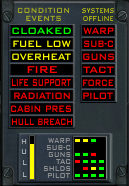
\includegraphics[scale=0.70]{images/indicators.png}

SYSTEM INDICATORS: 
The system indicators are broken down in to several categories, namely
condition events, offline systems, hull status and system status.

Each parts rail of every system will be displayed as a green, yellow or red
indicator in the system status window depending on their status.  An
offline rail (one with a broken or missing part) will not be illuminated.
If all rails are offline, the functionality of that system is considered
offline and a red indicator light will illuminate in the "SYSTEMS OFFLINE"
indicator panel.

HULL INDICATOR BAR:
The "HULL" indicator shows the current state of the hull up to 100%.
Between 95-100\%, the indicator will be green (0, 255, 0, 255),
yellow between 30-94\%, otherwise red.  If the hull gets to 0\%, the
space ship is destroyed.  

CONDITION EVENTS
The condition events panel has illuminated text alerts that light upon a specific event. This text can be a graphic or a programically added font. These messages are, from top to bottom:

CLOAKED: (GREEN) Indicates Sundog is cloaked. 
FUEL LOW: (YELLOW) The "FUEL LOW" indicator is illuminated when there are only 200 units
of fuel left total (from both the main tank and the aux tank).
FUEL DRY: (RED) Indicates out of fuel. 
HULL BREACH: (RED) Lights when the hull state is below 10%. 

The other spaces may be used in the future for other conditions or alerts. 
 

%\begin{inparaenum}[\itshape a\upshape\)]
%\item condition events;
%\item offline systems;
%\item hull status; and
%\item system status
%\end{inparaenum}

Open Issues:
\begin{itemize}
\item In the mockup it says "FORCE" instead of "SHLDS" for the system
offline indicator.  Do we care about this (maybe we leave it as a cute
quirk)? (I'd rather we change FORCE to either SHLDS or SHIELDS (if SHIELDS can fit)). 
\end{itemize}

\subsection{System Bays}
The SunDog contains a number of system bays which control various aspects of
the ships' functionality.  Each of the bays require certain parts which are
necessary for the smooth operation of each individual system.  From time to
time, various parts will wear out or will become inoperative during certain
high stress times such as ship-to-ship combat.  If enough parts of a particular
system have been damaged, the system will go offline and will have to be
repaired.  This can create some potentially difficult situations if the
SunDog is engaged in combat and systems like shields or guns become
inoperative.  It is highly beneficial to have an extra supply of parts in
case things go wrong!

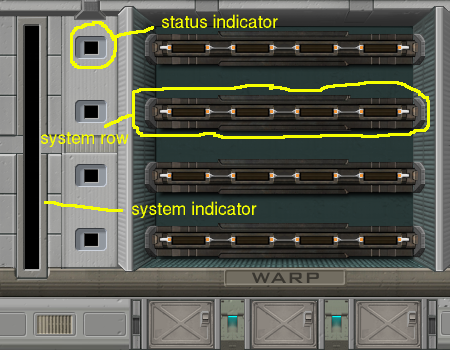
\includegraphics[scale=0.70]{images/interior-warp.png}

Each system bay contains four rows of parts, and each row can take a
combination of parts which is unique to that system bay.  Each row of
parts contributes 1/4 of the capability of a given system and all parts
in a given row need to be functioning for the row to work.

System parts are modular and can be plugged in to any slot that accepts the
same part.  Most slots can also take a "shunt", which is a universal part
which will allow the row to function, but in a reduced capacity.  Shunts
also have an uncanny ability to fail when they are most needed, so the use
of shunts should probably be avoided unless necessary.

A status row next to each system row indicates the current performance
of that row.  A green light indicates that the row is operating at
100\% capacity.  If a shunt is used for any part in the row, the row will
operate at 76\% capacity and the indicator light will be yellow.  If
more than one shunt is used in the row, the indicator light will be red
and the row output will be 48\% for two shunts and 24\% for three shunts.

\subsubsection{Pilotage}

\begin{tabular}{ | p{2.5cm} | p{2.5cm} | p{2.5cm} | p{2.5cm} | }
\hline
Slot 1 & Slot 2 & Slot 3 & Slot 4 \\ \hline
Control Node & J-Junc Module & Scanner & J-Junc Module \\
& Shunt & Shunt & Shunt \\
& & Ground Scanner & \\
\hline
\end{tabular}

Pilotage contains the ship's control and navigation systems. Without this system, the ship cannot use maps or fly.

\subsubsection{Guns}

\begin{tabular}{ | p{2.5cm} | p{2.5cm} | p{2.5cm} | p{2.5cm} | }
\hline
Slot 1 & Slot 2 & Slot 3 & Slot 4 \\ \hline
Control Node & Cryo Fuse & Photon Bridge & Plasma Tube \\
& Shunt & Shunt & Shunt \\
& Cloaker & & \\
\hline
\end{tabular}

The gun bay controls the operation of the cannon and laser systems aboard
the SunDog.  Without working guns the SunDog it is impossible to strike
back at attacking ships during ship-to-ship combat.

The lower the health of the gun system, the weaker the laser. The health bar of the system (as displayed in the system bay) shows health from 1-100%. This should coorespond to laser power. A system running at 83% will have a laser that is 83% of maximum power. The guns will also recharge slower.  At full health, the guns will recharge from 0 to 100% in three seconds. For every percent that the gun system has lost health, a tenth of a second should be added to the recharge time. For example: a gun system running at 80% health because of shunts in the system will have a five second recharge time - three seconds base recharge plus two seconds from the 20% loss of health. 

The laser is more powerful, but it is harder to hit the enemy ship. Conversely the cannon is easier to hit since the shells explode when in proximity to the enemy ship (they do not have to be a direct hit to deliver damage) but they are weaker. 

A laser hit should do 100 damage and a cannon should do 60 damage. (In the future, it may be good to have different types of laser frequencies and cannon shells, which can be selected in the TAC menu.) 



\subsubsection{Shields}

\begin{tabular}{ | p{2.5cm} | p{2.5cm} | p{2.5cm} | p{2.5cm} | }
\hline
Slot 1 & Slot 2 & Slot 3 & Slot 4 \\ \hline
Control Node & Cryo Fuse & Flux Modulator & Flux Modulator \\
& Shunt & Shunt & Shunt \\
& Cloaker & & \\
\hline
\end{tabular}

The shields system controls the ships shields which prevent damage to
the hull and system parts when the SunDog is under attack.  Without
properly working shields the SunDog will become damaged very quickly
if it takes a direct hit from enemy cannon or laser fire.

Open Issues:
\begin{itemize}
\item How does the shield efficiency affect the operation of the shields?
Presumably the efficiency determines the percentage to what the shields can
be raised to:  ie. 100\% efficiency and the shields can be raised 100\%.
With shields at 25\%, they could only be raised 25\%.
\item How does the shield efficiency determine the rate of damage?
\end{itemize}

\subsubsection{Sub-C}

\begin{tabular}{ | p{2.5cm} | p{2.5cm} | p{2.5cm} | p{2.5cm} | }
\hline
Slot 1 & Slot 2 & Slot 3 & Slot 4 \\ \hline
Control Node & Flux Modulator & ST Distorter & Cryo Fuse\\
& Shunt & Shunt & Shunt \\
\hline
\end{tabular}

Open Issues:
\begin{itemize}
\item Is the sub-light speed directly proportional to the efficiency
of the engines?  ie. if the system is at 75\% capacity, will it take
133\% as much time to arrive as it would if the engines were working at
100\%?
\end{itemize}

\subsubsection{Tactical}

\begin{tabular}{ | p{2.5cm} | p{2.5cm} | p{2.5cm} | p{2.5cm} | }
\hline
Slot 1 & Slot 2 & Slot 3 & Slot 4 \\ \hline
Control Node & Scanner & J-Junc Module & Photon Bridge \\
& Shunt & Shunt & Shunt \\
\hline
\end{tabular}

Open Issues:
\begin{itemize}
\item Presumably tactical would adversely affect the way the thrusters
work when maneuvering during combat.  Is there any other affect?
\end{itemize}

\subsubsection{Warp}

\begin{tabular}{ | p{2.5cm} | p{2.5cm} | p{2.5cm} | p{2.5cm} | }
\hline
Slot 1 & Slot 2 & Slot 3 & Slot 4 \\ \hline
Control Node & Flux Modulator & Photon Bridge & ST Distorter \\
& Shunt & Shunt & Shunt \\
\hline
\end{tabular}

Open Issues:
\begin{itemize}
\item Do the warp engines only determine the distance that the SunDog
can jump?  ie. if you have only one system row working, can the SunDog
only jump 1/4 the distance?
\end{itemize}

